\input{preamble}

\begin{document}

\title{Research Journal}
\maketitle

\phantomsection
\label{section-phantom}

\tableofcontents


\section{Toy deformations}
\label{section-toy-deformations}

In this section I will do some practice examples deforming simple schemes like
the twisted cubic.



\subsection{Last entry (June 2)}
\label{subsection-june-2}

On Thursday I had a meeting with Sergey where he explained more details about
how to do deformations using weights and how this translates to the resolution.
It will take me some time to metabolize this discussion and I have to go super
RG this month since exam is coming soon. After that RG course is over and I'll
be much more available. But still I'll try to start the digestion of how to do
deformations using weights. The \textbf{objective} is to get super good practice
and acquaintance doing simple examples (the twisted cubic deforms to SR of three
lines, this was the first nontrivial example of the deformation of a
non-complete intersection, remember? after triangle and pentagon…).

So basically just \textit{really} understand how to get from a twisted cubic to
SR of three lines would be good enough for a next meeting---probably not
tomorrow.

Here's what happened:
\begin{figure}[H]
\centering
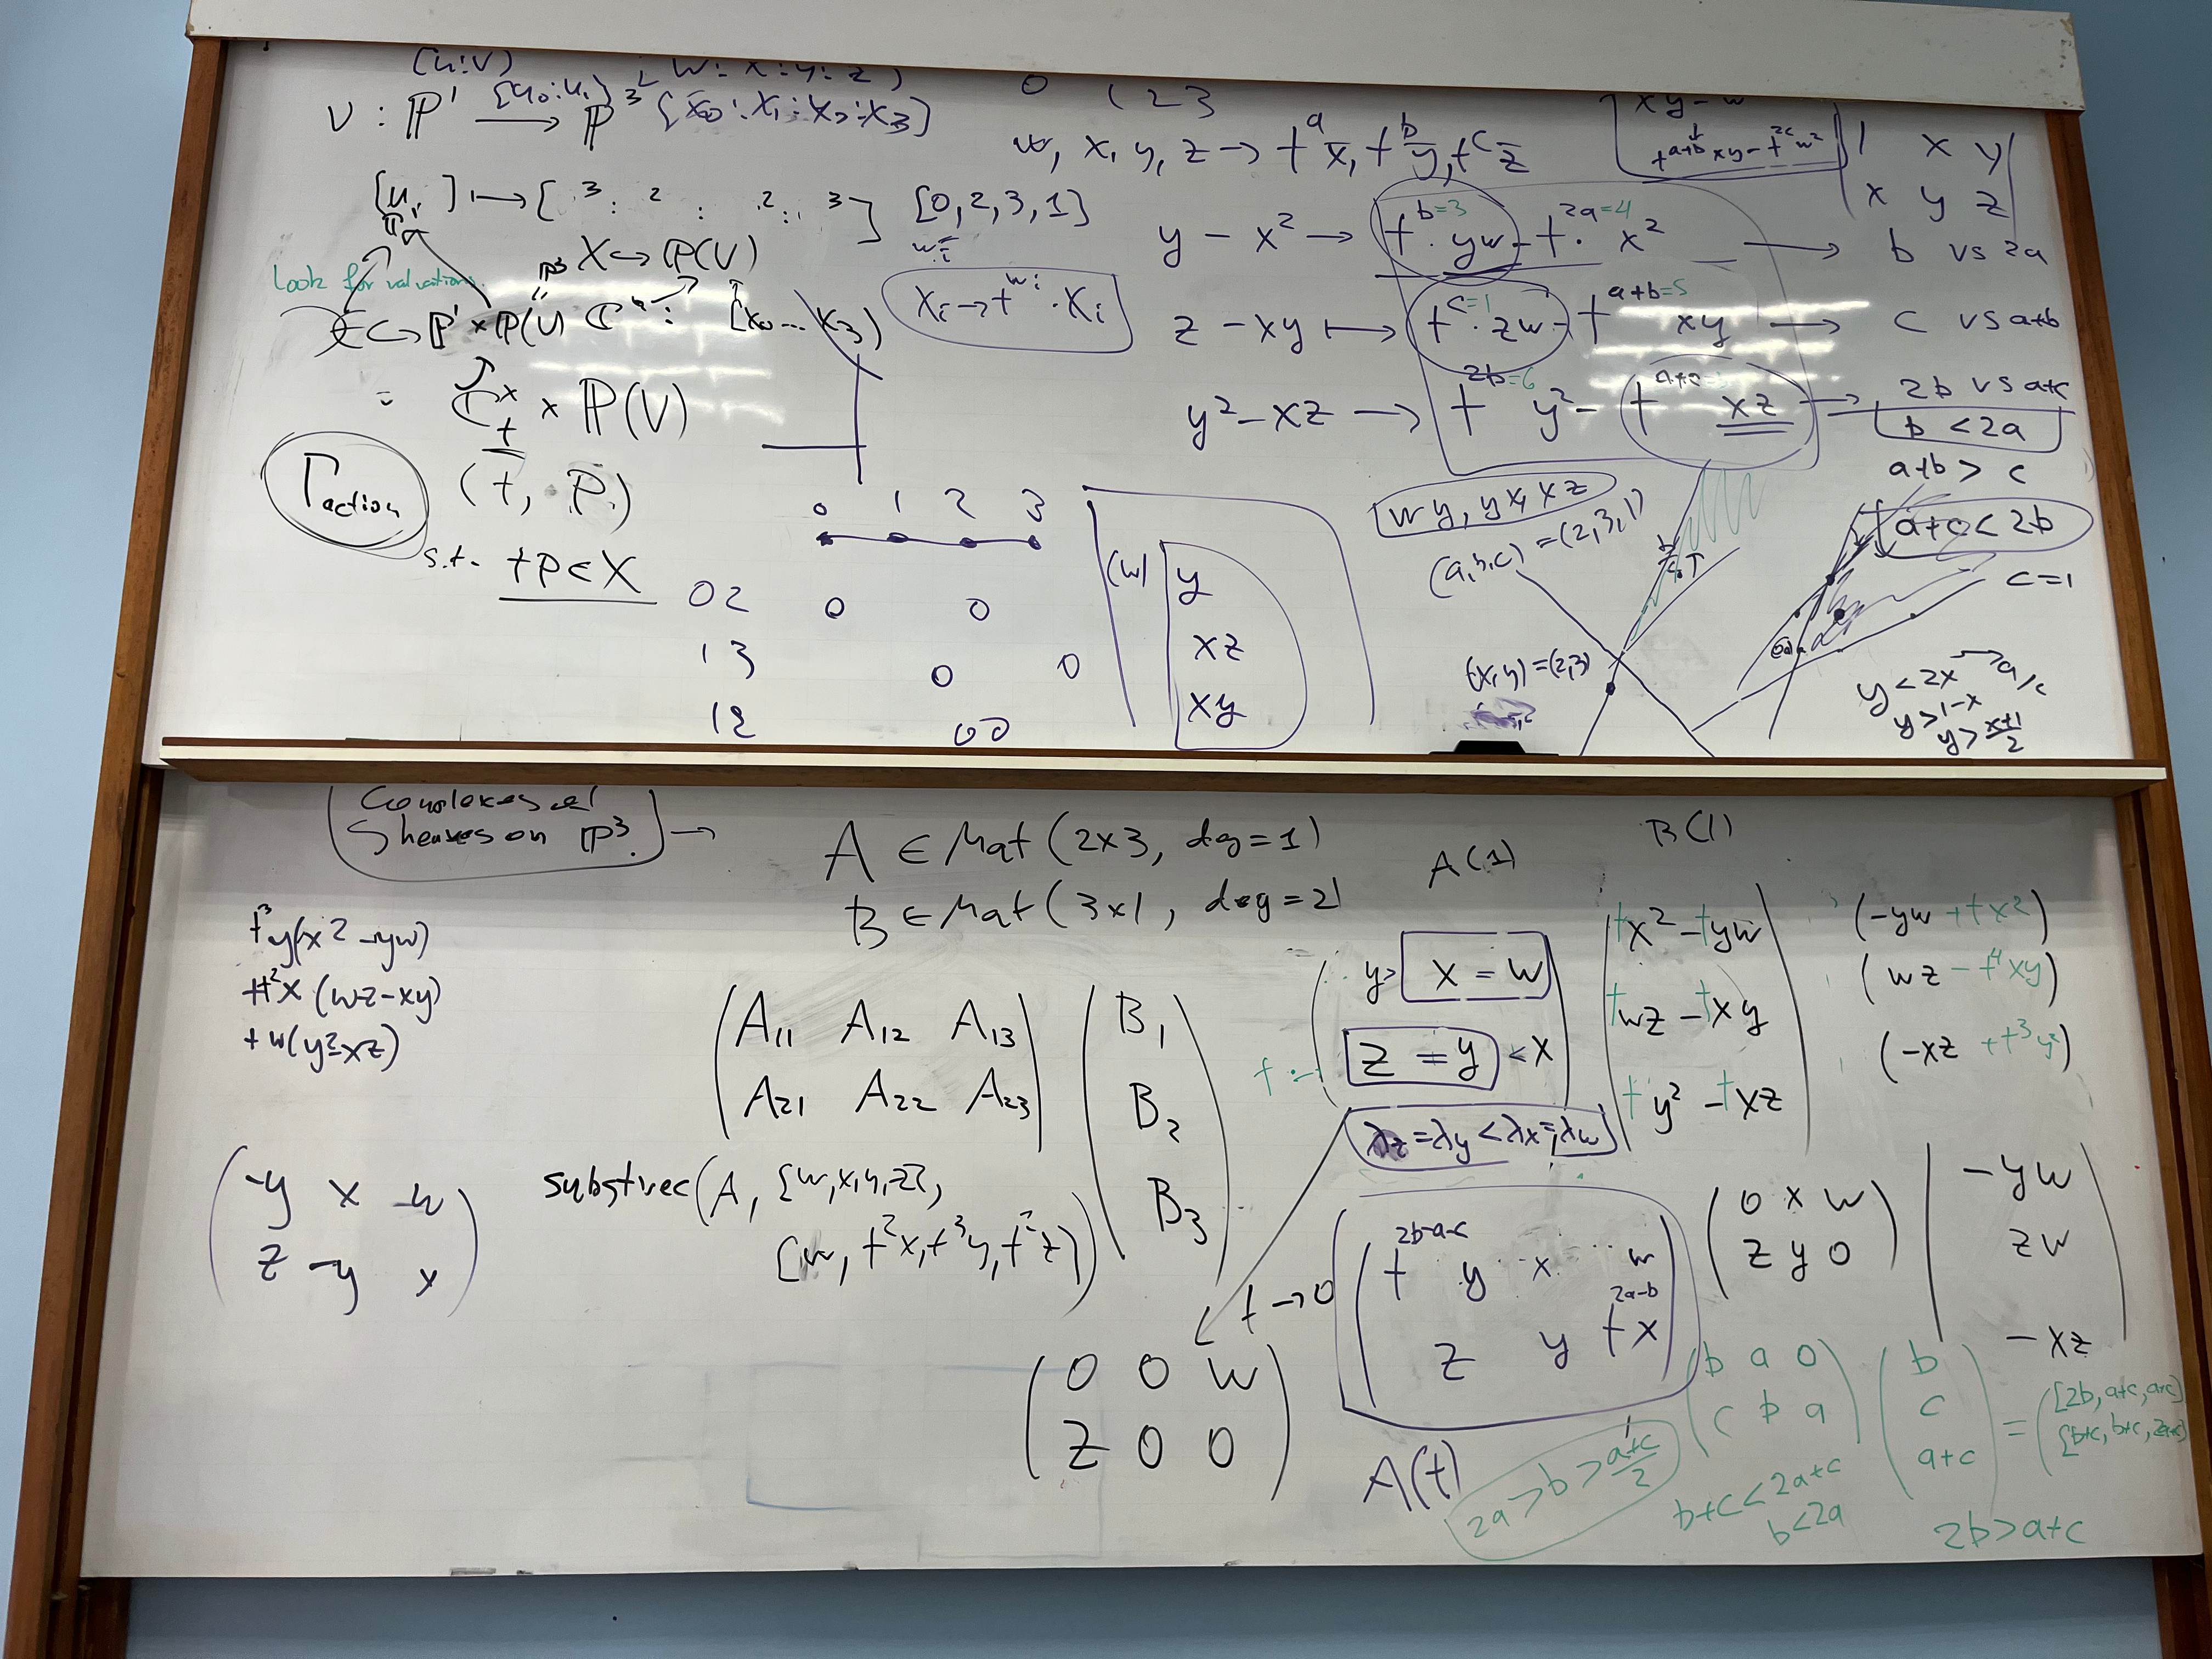
\includegraphics[width=1\textwidth]{figures/toy-deformations-board}
\label{figure-toy-deformations-board}
\end{figure}

\begin{definition}
\label{definition-twisted-cubic}
The {\it twisted cubic} is the image of the Veronesse map of degree 3,
\begin{align*}
\nu: \mathbb{P}^1 &\longrightarrow \mathbb{P}^3 \\
[u:v] &\longmapsto [x_0:x_1:x_2:x_3]
\end{align*}
\end{definition}

\begin{lemma}
\label{lemma-twisted-cubic-is-variety}
\begin{reference}
\cite[Proposition 6.1]{sys}
\end{reference}
The twisted cubic is an algebraic variety whose ideal is generated by the minors
of the matrix
$$
M_{3,1}=\begin{pmatrix}
x_0 & x_2 & x_3\\
x_1 & x_4 & x_0
\end{pmatrix}
$$
\end{lemma}

\begin{proof}
See \cite[Proposition 6.1]{sys}.
\end{proof}

Thus, the ideal of the twisted cubic is generated by
\begin{align}
\label{equation-twisted-cubic1}
x_0x_3&-x_1x_2\\
x_0^2&-x_3x_1\\
x_2x_0&-x_3^2
\end{align}

To understand the deformations we replace
$$
x_0\rightsquigarrow t^ax_0,x_1\rightsquigarrow t^bx_1,
x_2\rightsquigarrow t^cx_2,x_3\rightsquigarrow t^cx_3
$$
So that \ref{equation-twisted-cubic1} become
\begin{align}
\label{equation-twisted-cubic2}
t^{a+d}x_0x_3&-t^{b+c}x_1x_2\\
t^{2a}x_0t^{d+b}2&-x_3x_1\\
t^{c+a}x_2x_0&-t^{2d}x_3^2
\end{align}

\section{Deforming Grünbraum sphere}
\label{section-grunbaum-sphere}

Here I try to deform Grünbraum sphere.

\section{Twistor spaces}
\label{section-twistor-spaces}

Objectives:
\begin{enumerate}
\item Define twistor space.
\item Define de Sitter space.
\item How is Segre embedding working in this story?
\item What are magnetic monopoles?
\end{enumerate}

\begin{definition}[Twistor space]
\label{definition-twistor-space}
It's the space of compatible quaternionic structures $(I,J,K)$ on a complex
manifold. In some simple case it's $\mathbb{C}P^{1}$.
\end{definition}

The twistor space of Anti-de-Sitter space is
$$
\text{Tw}(\text{AdS}^3)=\mathbb{D}\times \mathbb{D}
$$
There is a natural quadratic form of signature $(2,2)$ on
$\mathbb{R}^4=\mathbb{R}^2 \otimes \mathbb{R}^2$. 

Now projectivize:
$$
\mathbb{P}^3=\mathbb{P}(\mathbb{R}^{2,2},Q)
$$
Now consider the hypersurface in $\mathbb{R}^4$ given by $Q(u)=1$. When we
projectivize we realize that the projectivization of the hypersurface is given
by those vectors where $Q$ is positive as a form restricted to the line
generated by that vector.

Anti de Sitter is the space where $Q>0$ in $\mathbb{R}^4$. Topologically it is a
product of spheres $S^{p-1}\times \mathbb{R}^q$. We can produce a metric by
consider the function:
$$
F(u):=\text{log}Q(u)
$$
then
$$
\mu \mapsto  \text{log}\det\mu
$$
and then it's Hessian $\partial_i \partial_j \text{log}\det \mu$.

Three perspectives… The symmetries of $\mathbb{D}$ are those which preserve the
 hermitian metric $|z|^2+|w|^2$… This allows to see the twistor space
 as a homogeneous space.

\section{Bridgeland Stability}
\label{section-Bridgeland-stability}

{\bf Objectives}
\begin{enumerate}
\item What is the $(\alpha,\beta)$-plane from \cite{wall-crossing}? Knowing this
is crucial for understanding the picture.
\item What is an instanton?
\end{enumerate}

\section{Quantum Cohomology}
\label{section-quantum-cohomology}

\subsection{Galkin seminar (June 20 2025)}
\label{subsection-Galkin-June-20}

{\bf Question.} Is it true that quantum cohomology is just simplicial cohomology
classes with coefficients in $\mathbb{C}$ but with a different product?

{\bf A.} (Adapted from Sergey's.) We extend the coefficients from $\mathbb{C}$
to $\mathbb{C}[q]$ where $q$ is ``a formal variable''. So as a
$\mathbb{C}[q]$-module ($HQ^*(X)$) this is the ``usual'' cohomology, but the
product is not the cup product (however it coincides with cup-product module the
ideal $(q)$).

\begin{quotation}
``Then geometrically you take Spec of such algebra and it
fibers over $\text{Spec} \mathbb{C}[q] = A^1_\mathbb{C}$ with coordinate q
(alias, any element of a commutative algebra can be consideredf as a function
from its Spectrum to the affine line), and the you can take a fiber over any
point a, which is the same as substituting q to a value (complex number) a.
Functions on this fiber is the quotient algebra QH(X,a) = QH(X,C[q])/(q-a), the
structure constants are obtained by sybstituting q by a."
\end{quotation}

{\bf Question.} What is that fibered construction good for?


{\bf Theme.} Under what conditions $QH^{\text{ev}}_{\text{big}}(X)$ is
generically semisimple?

{\bf Results.} Odd Betti numbers and odd Hodge numbers will vanish. See
Hertling, Manin, Teleman 2009.

{\bf Beautiful question.} When is the cohomology $H^*(Y)$ of Hodge-Tate type,
where $Y$ is a generic hyperplane section of the complex Grassmanian
$\text{Gr}(n,k)$?

{\bf Reference + remark.} Debarre-Voisin computed the Hodge diamond of $Y
\subset \text{Gr}(3,10)$ when studying Hyper-Kähler fourfolds. Since this is not
Hodge-Tate type, the small quantum-cohomology is not generically semisimple.

\begin{theorem}[Galkin-Leung-L.-Xiong]
\label{theorem-GLLX}
For $\text{Gr}(k,n)$, the cohomology $H^{*}(Y)$ is of Hodge-Type if and only if
\begin{itemize}
\item $Y \subset \text{Gr}(1,n)\cong \text{Gr}(n-1,n)$ where $n\geq 1$.
\item $Y \subset \text{Gr}(2,n) \cong \text{Gr}(n-2,n)$ where $n \geq 4$.
\item $Y \subset\text{Gr}(3,n) \cong\text{Gr}(n-3,n)$ where $n=6,7,8$.
\end{itemize}
\end{theorem}

Theorem \ref{theorem-GLLX} can be viewed as an {\bf ADE classification}. We call
the above $Y$ a {\it Hodge-Tate hyperplane section}.

{\bf Reference.} Try it online
\url{https://cubicbear.github.io/PluckerHodge.html} 

For Fano varieties, we have the Fano index \ref{definition-Fano-index}. In this
case, $QH^*(X)|_{q=1}$ is naturally a $\mathbb{Z}_r$-graded algebra
$\mathcal{A}$.

\bibliography{my}
\bibliographystyle{amsalpha}

\end{document}
